% !TEX encoding = UTF-8 Unicode

\Chapter{Szűrő algoritmusok}
Ebben a fejezetben azokat a filtereket szeretném részletezni, amelyeket megírtam C++ progaramozási nyelven. Ezek többségükben cartoon, valamint festmény jellegűek. A szűrőket nem csak képeken teszteltem, hanem videókon is és valós időben is a számítógépem kamerájával, de azok eredményét majd a \textbf{6. fejezet}ben fogom bővebben kifejteni.
\Section{Cartoon-style filter}
Az első filter egy Cartoon-style filter, amely az éleket kiemeli és a színeket elmossa. Ezekhez a műveletekhez Gauss-piramist, kétoldalú szűrőést, medián szűrést illetve adaptív küszöbölést használtam.
\begin{figure}[ht]
\centering
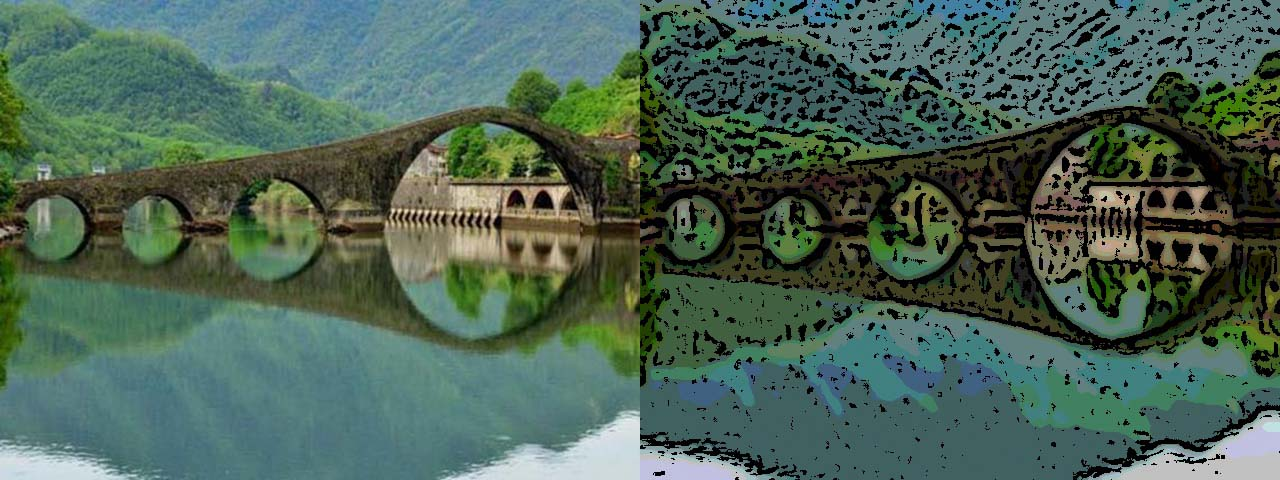
\epsfig{file=kepek/1_cartoon_filter.jpg, width=15cm, height=5.625cm}
\caption{Bal oldalon az eredeti kép látható, jobb oldalon a filterrel ellátott kép} 
\label{fig: cartoon1}
\end{figure}
\SubSection{1. lépés: Gauss-piramis és kétoldalú szűrő}
Első lépésben az eredeti képet lekicsinyítettem Gauss-piramis segítségével a kép méretének negyedére, rátettem egy kétoldalú szűrőt, majd vissza nagyítottam az eredeti méretre. A Gauss-piramis a kép kicsinyítése előtt Gauss-simítás segítségével súlyoz. A kétoldalú szűrő egy nem lineáris, élvédő és zajcsökkentő simító szűrő.
\begin{figure}[ht]
\centering
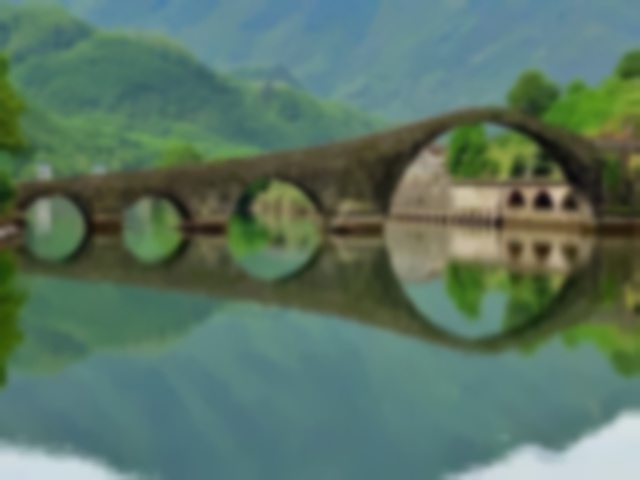
\epsfig{file=kepek/pyrambilateral.jpg,scale=0.45}
\caption{A Gauss-piramisban kicsinyítés és nagyítás valamint a kétoldalú szűrő eredménye } 
\label{fig: cartoon2}
\end{figure}
\SubSection{2. lépés: Medián szűrő}
Ebben a lépésben először az előzőleg kapott elmosott, színes képet átkonvertáltam szürkeárnyalatos képpé. Ennek eredményeként kapott képen medián szűrést hajtottam végre, amit ismét zajcsökkentés miatt alkalmaztam. Így a kép már teljesen el van mosva, egyre jobban cartoon hatása van.
\begin{figure}[ht]
\centering
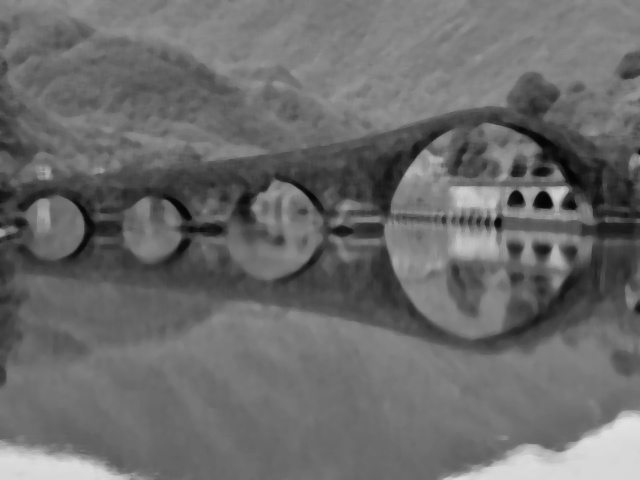
\epsfig{file=kepek/graymedian.jpg,scale=0.45}
\caption{Szürkére átalakított kép medián szűrővel } 
\label{fig: cartoon3}
\end{figure}
\SubSection{3. lépés: Adaptív küszöbölés az élek kiemelésére}
Az adaptív küszöbérték általában szürkeárnyalatos vagy színes képet ad bemenetként, és a legegyszerűbb megvalósításban bináris képet jelenít meg, amely szegmentálást jelent. A kép minden egyes képpontjára egy küszöbértéket kell kiszámítani. Ha a képpontérték a küszöbérték alatt van, akkor a háttérértékre van állítva, ellenkező esetben az előtérbe kerül.
\begin{figure}[ht]
\centering
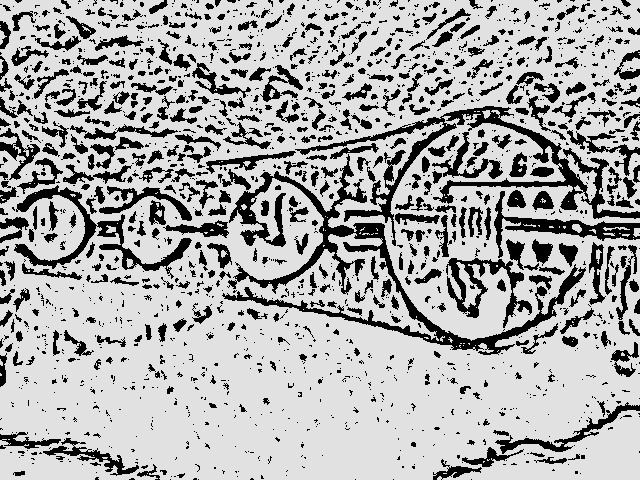
\epsfig{file=kepek/threshold.jpg,scale=0.40}
\caption{Adaptív küszöbölés  } 
\label{fig: cartoon4}
\end{figure}
\SubSection{4. lépés: A szűrőkkel és a köszöböléssel előállított képek eggyesítése}
Az adaptív küszöböléssel elkészült maszkot át kell konvertálni színes képpé, hogy egyesíteni tudjuk az "elmosott" képpel amit az első két lépésben hoztunk létre.
\begin{figure}[ht]
\centering
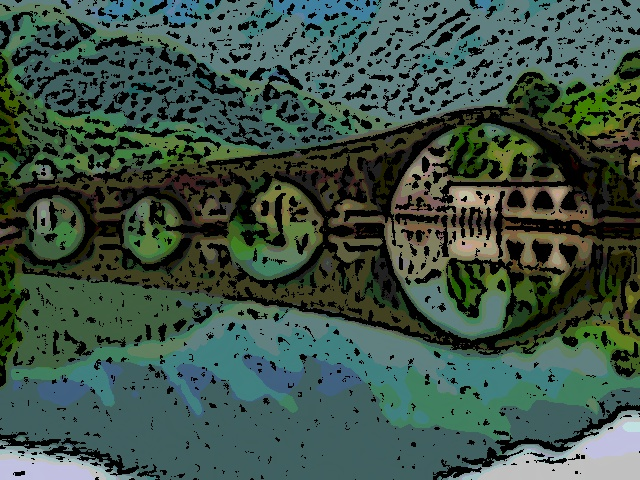
\epsfig{file=kepek/Cartoon_filter.jpg,scale=0.40}
\caption{Cartoon-style szűrő } 
\label{fig: cartoon5}
\end{figure}
\Section{Pencil sketch filter}
Megpróbáltam egy olyan algoritmust létrehozni, ami egy ceruza rajzot imitál. Ehhez szűrkeárnyalatosra konvertáltam a képet, Medián szűrőt, Gauss szűrőt és egyéb képfeldolgozási műveleteket használtam, valamint egy "vásznat" is ráraktam, hogy még jobban olyan érzete legyen a képnek mint ha rajzolták volna.
\begin{figure}[ht]
\centering
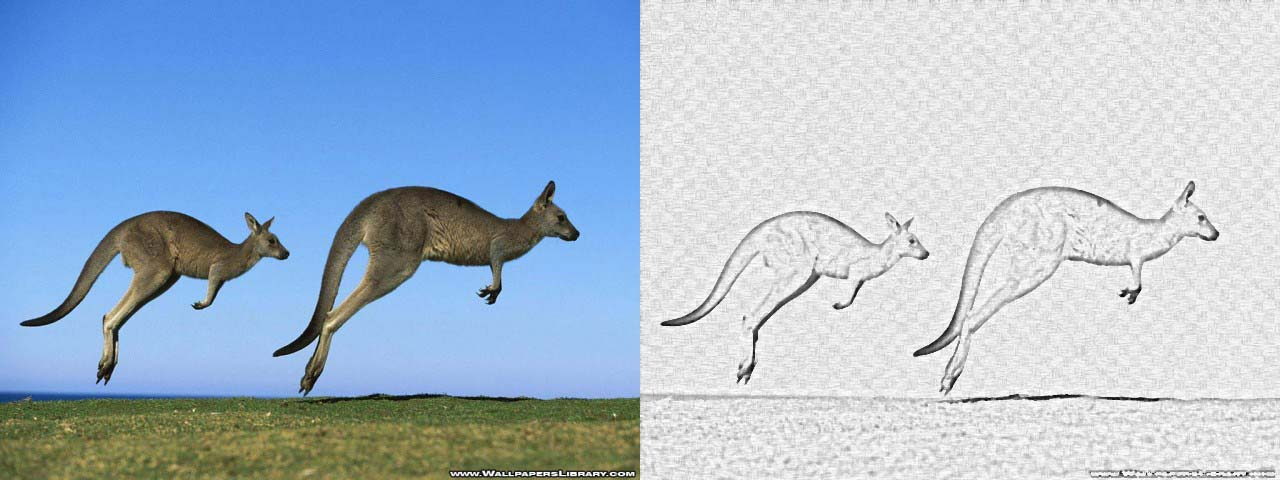
\epsfig{file=kepek/2_pencil_sketch_filter.jpg,width=15cm, height=5.625cm}
\caption{Bal oldalon az eredeti kép látható, jobb oldalon a filterrel ellátott kép } 
\label{fig: pencil1}
\end{figure}
\SubSection{1. lépés: Medián szűrő}
A kép szűrkeárnyalatos konvertálása után, végrehajtottam egy medián szűrést annak érdekében, hogy kiszűrjük az apróbb zajokat.
\begin{figure}[ht]
\centering
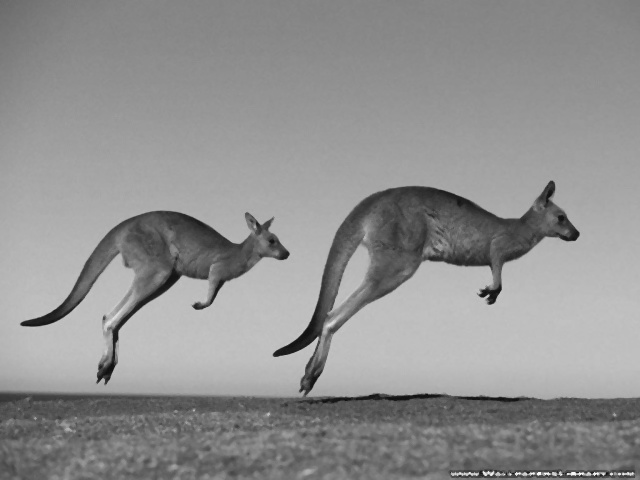
\epsfig{file=kepek/mediangray.jpg,scale=0.50}
\caption{Szürkére átalakított kép medián szűrővel  } 
\label{fig: pencil2}
\end{figure}
\SubSection{2. lépés: Gauss szűrő}
Ezt a simítási teknikát, a képzaj  és a részletesség csökkentése érdekében használtam. Olyan sima elmosódást eredményez a képen, mint ha a nem lenne fókuszban.
\begin{figure}[ht]
\centering
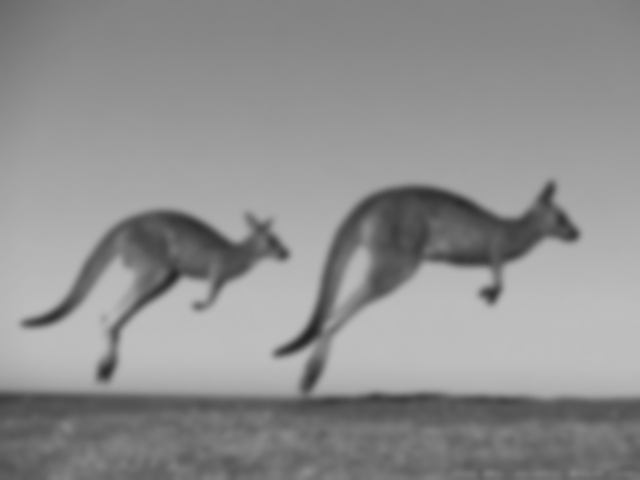
\epsfig{file=kepek/gauss.jpg,scale=0.43}
\caption{Gauss szűrő használata } 
\label{fig: pencil3}
\end{figure}
\SubSection{3. lépés: Az előző két lépés elosztása }
Az előző két szűrőt elosztottam egymással, így már tényleg majdnem olyan képet kaptam ami már ceruza rajz szerű. Úgy gondoltam még azért ráfér némi javítás, így még további műveleteket hajtottam végre rajta.
\begin{figure}[ht] 
\centering
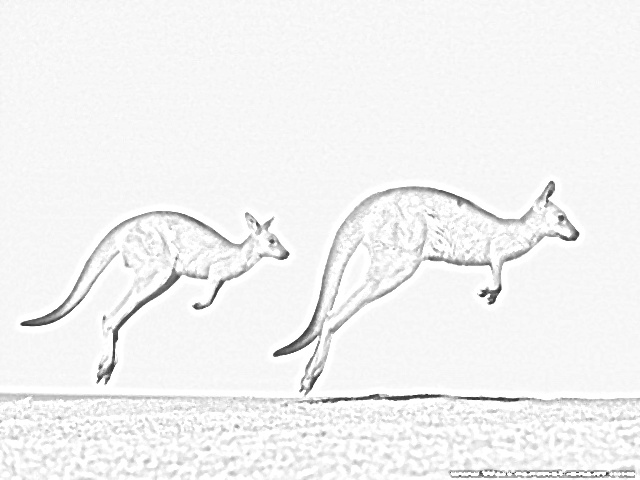
\epsfig{file=kepek/blend.jpg,scale=0.43}
\caption{Medián szűrés és a Gauss szűrés hányadosa } 
\label{fig: pencil4}
\end{figure}
\SubSection{4. lépés: Kontraszt széthúzása}
Azt figyeltem meg, hogy ha így hagyom a "Pencil sketch" szűrőt, akkor némely képen eléggé kontraszt szegény. Így úgy gondoltam rakok bele egy kontraszt széthúzást, hogy még kontrasztosabb legyen a kép.
\begin{figure}[ht]
\centering
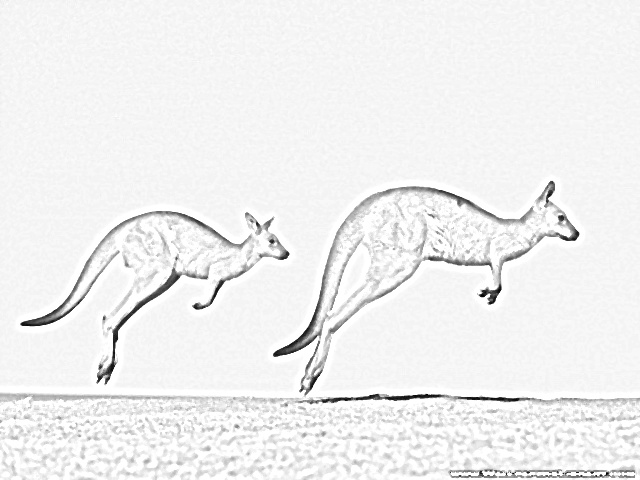
\epsfig{file=kepek/contraststrech.jpg,scale=0.50}
\caption{Kontraszt széthúzás } 
\label{fig: pencil5}
\end{figure}
\SubSection{5. lépés: Vászon hozzáadása}
A kontraszt széthúzása után, már egészen olyan hatása volt a képnek mint ha egy ceruza rajz lenne. Ráraktam még egy "vászont" ami személyes véleményem szerint mégjobban segíti azt az érzetet hogy ez egy ceruza rajz. Először a vászonnak a színét átkellett konvertálnom  színesből szűrkeárnyalatossá, hogy használható legyen a kontraszt széthúzott képhez. Ezek után a vászont összeszoroztam eddig eredményül kapott képpel így jött létre a "Pencil sketch filter".
\begin{figure}[ht] 
\centering

\epsfig{file=kepek/canvasgray.jpg,width=12cm, height=4cm}
\caption{Vászon színének konvertálása } 
\label{fig: pencil6}
\end{figure}
Így készült el végeredményként ez a kép.
\begin{figure}[ht]
\centering
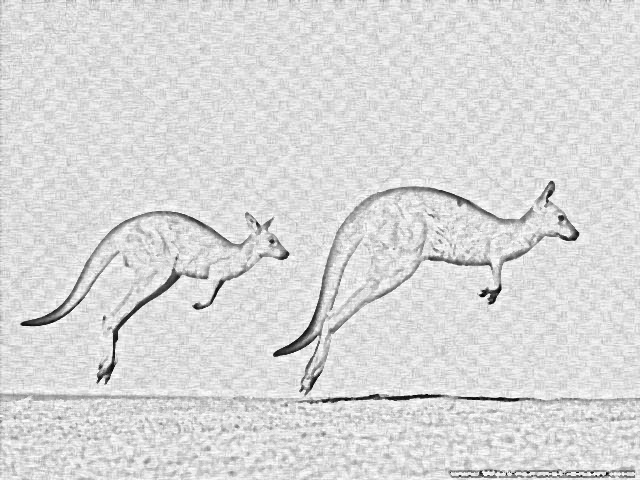
\epsfig{file=kepek/pencil_sketch.jpg, scale=0.50}
\caption{Pencil sketch filter } 
\label{fig: pencil7}
\end{figure}
\Section{Cartoon filter}
Megpróbáltam más technikával is létrehozni egy cartoon hatású képet. Ahol medián szűrőt, Laplacian éldetektálást valamit küszöbölést használtam.
\begin{figure}[ht]
\centering
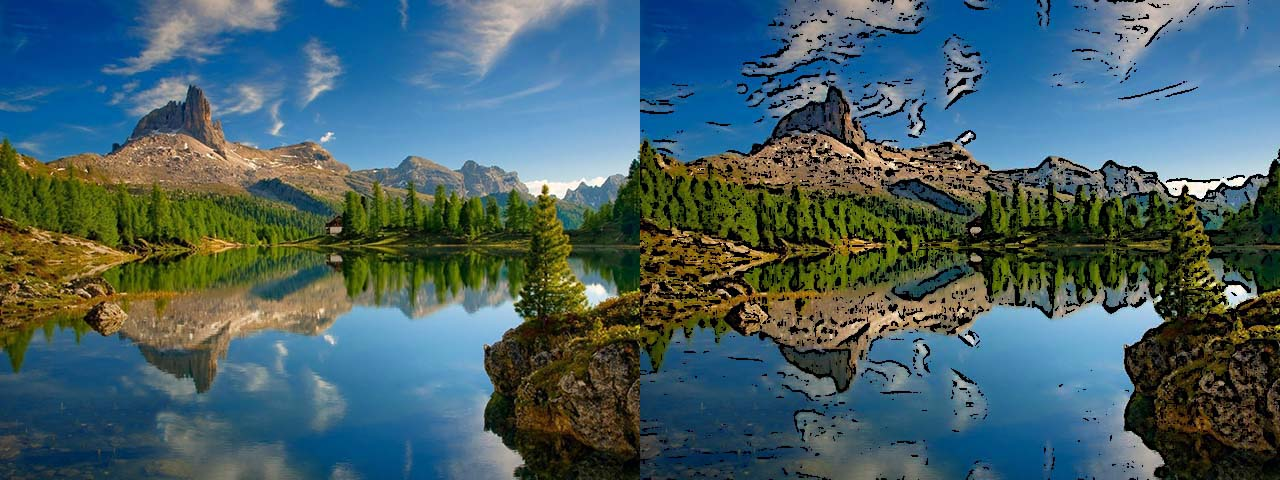
\epsfig{file=kepek/3_cartoon_filter2.jpg,width=15cm, height=5.625cm}
\caption{Bal oldalon az eredeti kép látható, jobb oldalon a filterrel ellátott kép } 
\label{fig: 2_cartoon1}
\end{figure}
\SubSection{1. lépés: Medián szűrő}
Mint az eddigi saját filtereknél itt is előfeldolgozásként elvégeztem szürkeárnyalatossá konvertálást és medián szűrést alkalmaztam. 
\begin{figure}[ht]
\centering
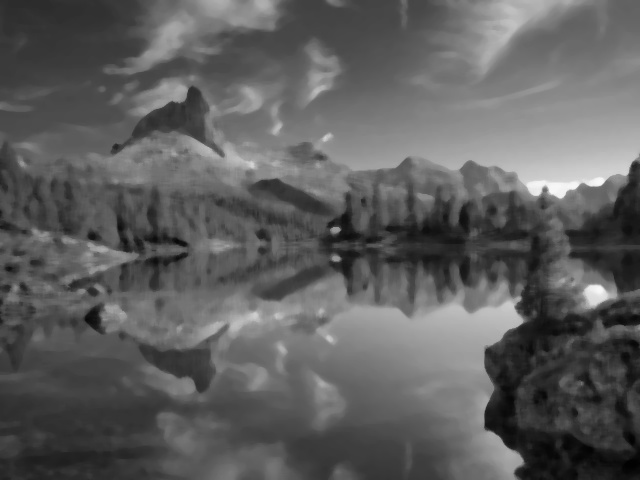
\epsfig{file=kepek/Cartoon1_gray.jpg,scale=0.485}
\caption{Szürkére átalakított kép medián szűrővel  } 
\label{fig:  2_cartoon2}
\end{figure}
\SubSection{2. lépés: Laplacian éldetektálás}
Ennél a filternél a Laplacian éldetektálást választottam, azért ezt a módszert mert ezzel olyan élmaszkot tudtam készíteni ami kicsit hasonló a ceruza rajzhoz. Vékony kontúrként emeli ki a képben található éleket. Ez az éldetektálás gradiensekkel számol, ahol a gradiens nagy, ott a második derivált 0.
\begin{figure}[ht]
\centering
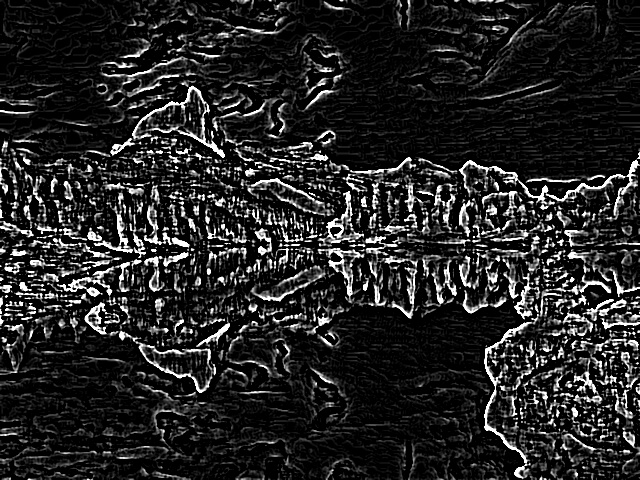
\epsfig{file=kepek/Cartoon1_laplacian.jpg,scale=0.485}
\caption{Laplacian éldetektálás  } 
\label{fig:  2_cartoon3}
\end{figure}
\SubSection{3. lépés: Küszöbölés}
Az éldetektálás után, alkalmaztam egy küszöbölést amivel létrejött egy maszk, amit összeraktam az eredeti képpel.
\begin{figure}[ht]
\centering
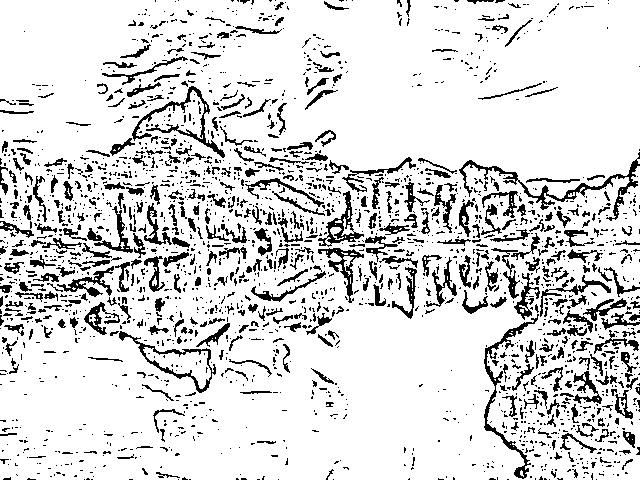
\epsfig{file=kepek/Cartoon1_thresh.jpg,scale=0.48}
\caption{Küszöbölés  } 
\label{fig:  2_cartoon4}
\end{figure}
Így készült el végeredményként a Cartoon filter.
\begin{figure}[ht]
\centering
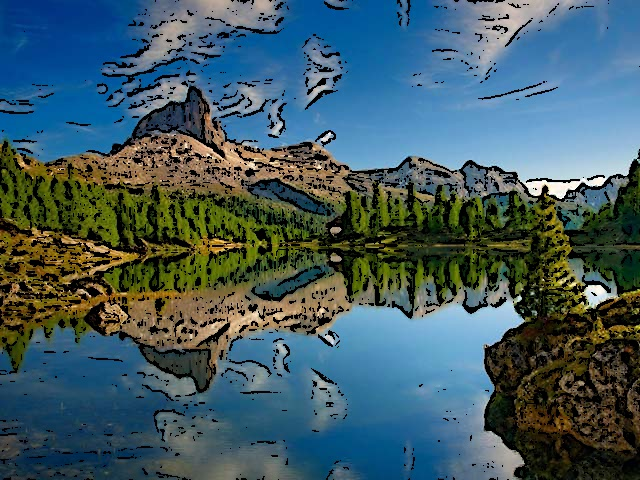
\epsfig{file=kepek/Cartoon1_filter1.jpg,scale=0.48}
\caption{Cartoon filter  } 
\label{fig:  2_cartoon4}
\end{figure}
\Section{Paint-style filter}
Az utolsó saját szűrő amit készítettem az egy egyszerű festmény hatású szűrő. Ez a szűrő teljesen más technikával készült mint az eddigiek. Nem használtam éldetektálást illettve küszöbölést sem. Az eredeti képpel dolgoztam végig nem maszkoltam. Azért is egyszerű mert igazából két lépéssel megoldható, elég egy átlagoló szűrés és egy mean shift szegmentálás.
\begin{figure}[ht]
\centering
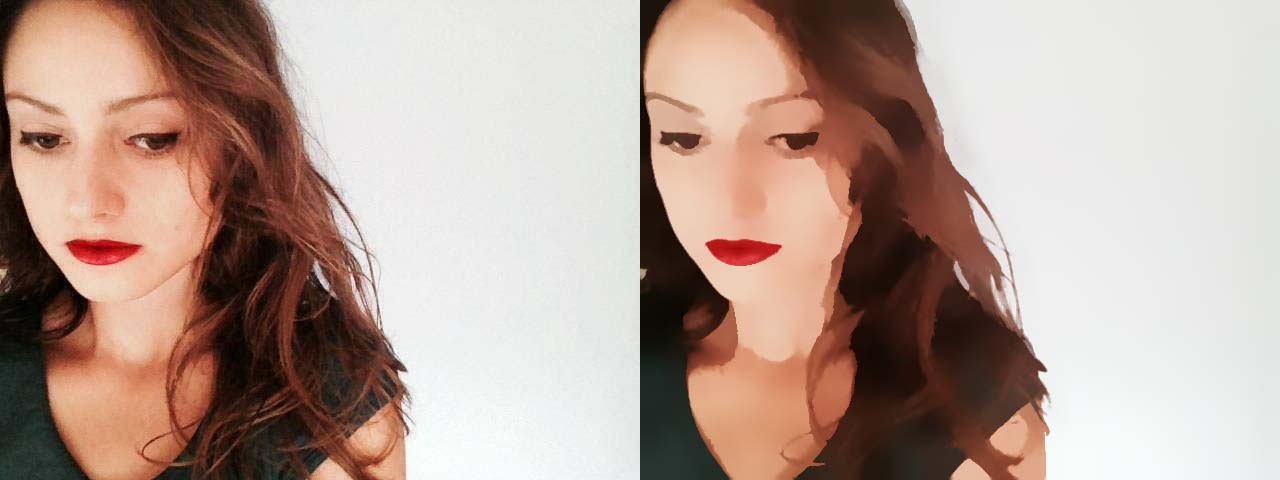
\epsfig{file=kepek/4_paint_filter.jpg,width=15cm, height=5.625cm}
\caption{Paint-style filter  } 
\label{fig:  paint}
\end{figure}
\SubSection{1. lépés: Átlagoló szűrő}
Átlagoló szűrővel elmostam az eredeti színes képet, hogy az apróbb zajokat kiszűrjem.
\begin{figure}[ht]
\centering
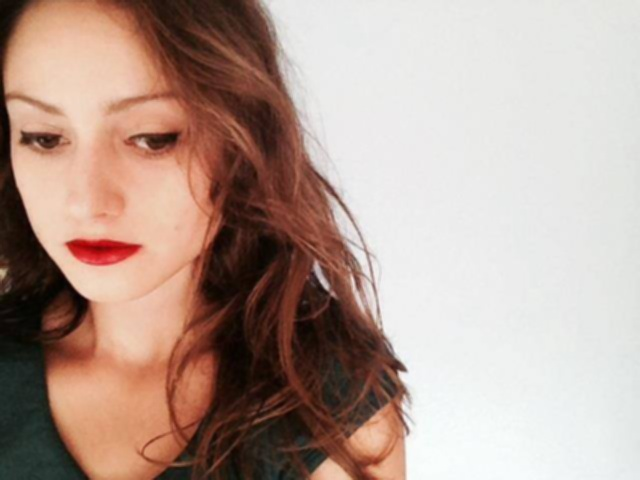
\epsfig{file=kepek/Paint_filter_blur.jpg,scale=0.48}
\caption{Átlagoló szűrő  } 
\label{fig: paint1}
\end{figure}
\SubSection{2. lépés: Mean shift szegmentálás }
Minden egyes adatpontnál a mean shift meghatároz egy ablakot, és kiszámítja az adatpont átlagát. Ezután az ablak közepét az átlag felé tolja, és megismétli az algoritmust, amíg konvergens. Az mean shift egy nemparametrikus iteratív algoritmus vagy egy nemparametrikus sűrűségi gradiens becslés egy általánosított kernel megközelítés alkalmazásával.
\begin{figure}[ht]
\centering
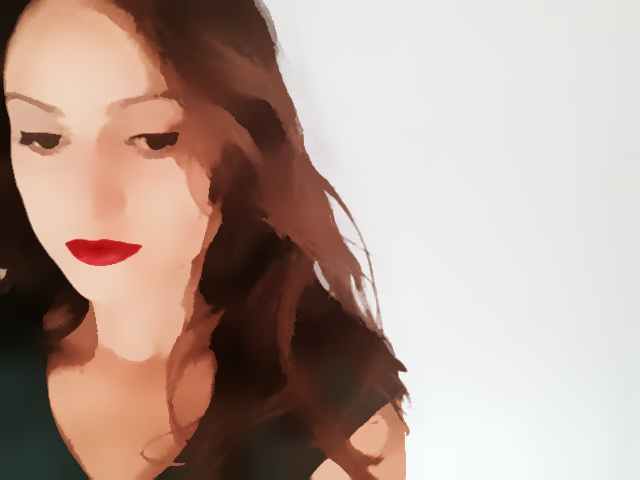
\epsfig{file=kepek/Paint_filter.jpg,scale=0.48}
\caption{Paint-stye filter, mean shift szegmentálás  } 
\label{fig: paint1}
\end{figure}




% Ide kellene felsorolni majd a saját szűrők algoritmusait!